%-----------------------------------------------------------------------------------------
% Autor dieser Vorlage:
% Stefan Macke (http://fachinformatiker-anwendungsentwicklung.net)
% Permalink zur Vorlage: http://fiae.link/LaTeXVorlageFIAE
%
% Sämtliche verwendeten Abbildungen, Tabellen und Listings stammen von Dirk Grashorn.
%
% Lizenz: Creative Commons 4.0 Namensnennung - Weitergabe unter gleichen Bedingungen
% -----------------------------------------------------------------------------------------

\documentclass[
	ngerman,
	toc=listof, % Abbildungsverzeichnis sowie Tabellenverzeichnis in das Inhaltsverzeichnis aufnehmen
	toc=bibliography, % Literaturverzeichnis in das Inhaltsverzeichnis aufnehmen
	footnotes=multiple, % Trennen von direkt aufeinander folgenden Fußnoten
	parskip=half, % vertikalen Abstand zwischen Absätzen verwenden anstatt horizontale Einrückung von Folgeabsätzen
	numbers=noendperiod % Den letzten Punkt nach einer Nummerierung entfernen (nach DIN 5008)
]{scrartcl}
\usepackage{luatex85}
\pdfminorversion=5 % erlaubt das Einfügen von pdf-Dateien bis Version 1.7, ohne eine Fehlermeldung zu werfen (keine Garantie für fehlerfreies Einbetten!)
\usepackage[utf8]{inputenc} % muss als erstes eingebunden werden, da Meta/Packages ggfs. Sonderzeichen enthalten

% !TEX root = Projektdokumentation.tex

% Hinweis: der Titel muss zum Inhalt des Projekts passen und den zentralen Inhalt des Projekts deutlich herausstellen
\newcommand{\titel}{Entwicklung von NatInfo}
\newcommand{\untertitel}{Webbasiertes Tool zur Unterstützung der Entwickler}
\newcommand{\kompletterTitel}{\titel{} -- \untertitel}

\newcommand{\autorName}{Stefan Macke}
\newcommand{\autorAnschrift}{Meine Straße 1}
\newcommand{\autorOrt}{49377 Vechta}

\newcommand{\betriebLogo}{LogoBetrieb.pdf}
\newcommand{\betriebName}{\textsc{Alte Oldenburger} Krankenversicherung AG}
\newcommand{\betriebAnschrift}{Alte-Oldenburger-Platz 1}
\newcommand{\betriebOrt}{49377 Vechta}

\newcommand{\ausbildungsberuf}{Fachinformatiker für Anwendungsentwicklung}
\newcommand{\betreff}{Dokumentation zur betrieblichen Projektarbeit}
\newcommand{\pruefungstermin}{Sommer 2015}
\newcommand{\abgabeOrt}{Vechta}
\newcommand{\abgabeTermin}{23.04.2015}
 % Metadaten zu diesem Dokument (Autor usw.)
% !TEX root = ../Projektdokumentation.tex

% Anpassung an Landessprache ---------------------------------------------------
\usepackage{babel}

% Umlaute ----------------------------------------------------------------------
%   Umlaute/Sonderzeichen wie äüöß direkt im Quelltext verwenden (CodePage).
%   Erlaubt automatische Trennung von Worten mit Umlauten.
% ------------------------------------------------------------------------------
%\usepackage[T1]{fontenc}
%\usepackage{textcomp} % Euro-Zeichen etc.

% Schrift ----------------------------------------------------------------------
% \usepackage{lmodern} % bessere Fonts
\usepackage{fontspec}
\setmainfont[
BoldFont=arialbd.ttf,
ItalicFont=ariali.ttf,
BoldItalicFont=arialbi.ttf,
]{arial.ttf} % Arial als Font
\usepackage{relsize} % Schriftgröße relativ festlegen

% Tabellen ---------------------------------------------------------------------
\PassOptionsToPackage{table}{xcolor}
\usepackage{tabularx}
% für lange Tabellen
\usepackage{longtable}
\usepackage{array}
\usepackage{ragged2e}
\usepackage{lscape}
\newcolumntype{w}[1]{>{\raggedleft\hspace{0pt}}p{#1}} % Spaltendefinition rechtsbündig mit definierter Breite

% Grafiken ---------------------------------------------------------------------
\usepackage[dvips,final]{graphicx} % Einbinden von JPG-Grafiken ermöglichen
\usepackage{graphics} % keepaspectratio
\usepackage{floatflt} % zum Umfließen von Bildern
\graphicspath{{Bilder/}} % hier liegen die Bilder des Dokuments

% Sonstiges --------------------------------------------------------------------
\usepackage[titles]{tocloft} % Inhaltsverzeichnis DIN 5008 gerecht einrücken
\usepackage{amsmath,amsfonts} % Befehle aus AMSTeX für mathematische Symbole
\usepackage{enumitem} % anpassbare Enumerates/Itemizes
\usepackage{xspace} % sorgt dafür, dass Leerzeichen hinter parameterlosen Makros nicht als Makroendezeichen interpretiert werden

\usepackage{makeidx} % für Index-Ausgabe mit \printindex
\usepackage[printonlyused,nohyperlinks]{acronym} % es werden nur benutzte Definitionen aufgelistet

% Einfache Definition der Zeilenabstände und Seitenränder etc.
\usepackage{setspace}
\usepackage{geometry}

% Symbolverzeichnis
\usepackage[intoc]{nomencl}
\let\abbrev\nomenclature
\renewcommand{\nomname}{Abkürzungsverzeichnis}
\setlength{\nomlabelwidth}{.25\hsize}
\renewcommand{\nomlabel}[1]{#1 \dotfill}
\setlength{\nomitemsep}{-\parsep}

\usepackage{varioref} % Elegantere Verweise. „auf der nächsten Seite“
\usepackage{url} % URL verlinken, lange URLs umbrechen etc.

\usepackage{chngcntr} % fortlaufendes Durchnummerieren der Fußnoten
% \usepackage[perpage]{footmisc} % Alternative: Nummerierung der Fußnoten auf jeder Seite neu

\usepackage{ifthen} % bei der Definition eigener Befehle benötigt
\usepackage{todonotes} % definiert u.a. die Befehle \todo und \listoftodos
\usepackage[square]{natbib} % wichtig für korrekte Zitierweise

% PDF-Optionen -----------------------------------------------------------------
\usepackage{pdfpages}
\pdfminorversion=5 % erlaubt das Einfügen von pdf-Dateien bis Version 1.7, ohne eine Fehlermeldung zu werfen (keine Garantie für fehlerfreies Einbetten!)
\usepackage[
    bookmarks,
    bookmarksnumbered,
    bookmarksopen=true,
    bookmarksopenlevel=1,
    colorlinks=true,
% diese Farbdefinitionen zeichnen Links im PDF farblich aus
    anchorcolor=LinkColor,% Ankertext
    citecolor=LinkColor, % Verweise auf Literaturverzeichniseinträge im Text
    filecolor=LinkColor, % Verknüpfungen, die lokale Dateien öffnen
    menucolor=LinkColor, % Acrobat-Menüpunkte
    urlcolor=LinkColor,
% diese Farbdefinitionen sollten für den Druck verwendet werden (alles schwarz)
    %linkcolor=black, % einfache interne Verknüpfungen
    %anchorcolor=black, % Ankertext
    %citecolor=black, % Verweise auf Literaturverzeichniseinträge im Text
    %filecolor=black, % Verknüpfungen, die lokale Dateien öffnen
    %menucolor=black, % Acrobat-Menüpunkte
    %urlcolor=black,
%
    %backref, % Quellen werden zurück auf ihre Zitate verlinkt
    luatex,
    plainpages=false, % zur korrekten Erstellung der Bookmarks
    pdfpagelabels=true, % zur korrekten Erstellung der Bookmarks
    hypertexnames=false, % zur korrekten Erstellung der Bookmarks
    linkcolor=LinkColor,
    linktoc=page,
]{hyperref}
% Befehle, die Umlaute ausgeben, führen zu Fehlern, wenn sie hyperref als Optionen übergeben werden
\hypersetup{
    pdftitle={\titel},
    pdfauthor={\autorName},
    pdfcreator={\autorName},
    pdfsubject={\titel},
    pdfkeywords={\titel},
}


% zum Einbinden von Programmcode -----------------------------------------------
\usepackage{caption}
\usepackage[newfloat]{minted}
\SetupFloatingEnvironment{listing}{name=Listing, placement=hbp}
\renewcommand*{\listlistingname}{Listings}

\usepackage{xcolor}
\definecolor{hellgelb}{rgb}{1,1,0.9}
\definecolor{colKeys}{rgb}{0,0,1}
\definecolor{colIdentifier}{rgb}{0,0,0}
\definecolor{colComments}{rgb}{0,0.5,0}
\definecolor{colString}{rgb}{1,0,0}

% See https://pygments.org/styles/ or pygments -L styles
\usemintedstyle{sas}
\setminted{%
  bgcolor=hellgelb,%
  breaklines,%
  frame=single,%
  fontsize=\footnotesize,%
  linenos,%
  numbers=left,%
  numbersep=5pt,%
  tabsize=4,%
} % verwendete Packages
% !TEX root = ../Projektdokumentation.tex

% Seitenränder -----------------------------------------------------------------
\setlength{\topskip}{\ht\strutbox} % behebt Warnung von geometry
\geometry{a4paper,left=25mm,right=25mm,top=25mm,bottom=35mm}

\usepackage[
	automark, % Kapitelangaben in Kopfzeile automatisch erstellen
	headsepline, % Trennlinie unter Kopfzeile
	ilines % Trennlinie linksbündig ausrichten
]{scrlayer-scrpage}

% Kopf- und Fußzeilen ----------------------------------------------------------
\pagestyle{scrheadings}
% chapterpagestyle gibt es nicht in scrartcl
%\renewcommand{\chapterpagestyle}{scrheadings}
\clearscrheadfoot

% Kopfzeile
\renewcommand{\headfont}{\normalfont} % Schriftform der Kopfzeile
\ihead{\small{\titel} \\[2ex] \textit{\headmark}}
\chead{}
\ohead{\raisebox{-2mm}{\includegraphics[scale=0.25]{\betriebLogo}}}
\setlength{\headheight}{18mm} % Höhe der Kopfzeile
%\setheadwidth[0pt]{textwithmarginpar} % Kopfzeile über den Text hinaus verbreitern (falls Logo den Text überdeckt)

% Fußzeile
\ifoot{\autorName}
\cfoot{}
\ofoot{\pagemark}

% Überschriften nach DIN 5008 in einer Fluchtlinie
% ------------------------------------------------------------------------------

% Abstand zwischen Nummerierung und Überschrift definieren
% > Schön wäre hier die dynamische Berechnung des Abstandes in Abhängigkeit
% > der Verschachtelungstiefe des Inhaltsverzeichnisses
\newcommand{\headingSpace}{1.5cm}

% Abschnittsüberschriften im selben Stil wie beim Inhaltsverzeichnis einrücken
\renewcommand*{\othersectionlevelsformat}[3]{
  \makebox[\headingSpace][l]{#3\autodot}
}

% Für die Einrückung wird das Paket tocloft benötigt
%\cftsetindents{chapter}{0.0cm}{\headingSpace}
\cftsetindents{section}{0.0cm}{\headingSpace}
\cftsetindents{subsection}{0.0cm}{\headingSpace}
\cftsetindents{subsubsection}{0.0cm}{\headingSpace}
\cftsetindents{figure}{0.0cm}{\headingSpace}
\cftsetindents{table}{0.0cm}{\headingSpace}


% Allgemeines
% ------------------------------------------------------------------------------

\onehalfspacing % Zeilenabstand 1,5 Zeilen
\frenchspacing % erzeugt ein wenig mehr Platz hinter einem Punkt

% Schusterjungen und Hurenkinder vermeiden
\clubpenalty = 10000
\widowpenalty = 10000
\displaywidowpenalty = 10000

% Quellcode-Ausgabe formatieren
\lstset{numbers=left, numberstyle=\tiny, numbersep=5pt, breaklines=true}
\lstset{emph={square}, emphstyle=\color{red}, emph={[2]root,base}, emphstyle={[2]\color{blue}}}

\counterwithout{footnote}{section} % Fußnoten fortlaufend durchnummerieren
\setcounter{tocdepth}{3} % im Inhaltsverzeichnis werden die Kapitel bis zum Level der subsubsection übernommen
\setcounter{secnumdepth}{3} % Kapitel bis zum Level der subsubsection werden nummeriert

% Aufzählungen anpassen
\renewcommand{\labelenumi}{\arabic{enumi}.}
\renewcommand{\labelenumii}{\arabic{enumi}.\arabic{enumii}.}
\renewcommand{\labelenumiii}{\arabic{enumi}.\arabic{enumii}.\arabic{enumiii}}

% Tabellenfärbung:
\definecolor{heading}{rgb}{0.64,0.78,0.86}
\definecolor{odd}{rgb}{0.9,0.9,0.9}
 % Definitionen zum Aussehen der Seiten
% !TEX root = ../Projektdokumentation.tex

% Abkürzungen, ggfs. mit korrektem Leerraum
\newcommand{\bs}{$\backslash$\xspace}
\newcommand{\bspw}{bspw.\xspace}
\newcommand{\bzw}{bzw.\xspace}
\newcommand{\ca}{ca.\xspace}
\newcommand{\dahe}{\mbox{d.\,h.}\xspace}
\newcommand{\etc}{etc.\xspace}
\newcommand{\eur}[1]{\mbox{#1\,\texteuro}\xspace}
\newcommand{\evtl}{evtl.\xspace}
\newcommand{\ggfs}{ggfs.\xspace}
\newcommand{\Ggfs}{Ggfs.\xspace}
\newcommand{\gqq}[1]{\glqq{}#1\grqq{}}
\newcommand{\inkl}{inkl.\xspace}
\newcommand{\insb}{insb.\xspace}
\newcommand{\ua}{\mbox{u.\,a.}\xspace}
\newcommand{\usw}{usw.\xspace}
\newcommand{\Vgl}{Vgl.\xspace}
\newcommand{\zB}{\mbox{z.\,B.}\xspace}

% Befehle für häufig anfallende Aufgaben
\newcommand{\Abbildung}[1]{\autoref{fig:#1}}
\newcommand{\Anhang}[1]{\appendixname{}~\ref{#1}: \nameref{#1} \vpageref{#1}}
\newcommand{\includegraphicsKeepAspectRatio}[2]{\includegraphics[width=#2\textwidth,height=#2\textheight,keepaspectratio]{#1}}
\newcommand{\Zitat}[2][\empty]{\ifthenelse{\equal{#1}{\empty}}{\citep{#2}}{\citep[#1]{#2}}}
\newcommand{\Autor}[1]{\textsc{#1}} % zum Ausgeben von Autoren
\newcommand{\itemd}[2]{\item{\textbf{#1}}\\{#2}} % erzeugt ein Listenelement mit fetter Überschrift
\newcommand{\Verweis}[1]{\ref{#1} (\nameref{#1})}

% fügt Tabellen aus einer TEX-Datei ein
\newcommand{\tabelle}[3] % Parameter: caption, label, file
{\begin{table}[htbp]
\centering
\singlespacing
\input{Tabellen/#3}
\caption{#1}
\label{#2}
\end{table}}

\newcommand{\tabelleAnhang}[1] % Parameter: file
{\begin{center}
\singlespacing
\input{Tabellen/#1}
\end{center}}

% einfaches Wechseln der Schrift, z.B.: \changefont{cmss}{sbc}{n}
\newcommand{\changefont}[3]{\fontfamily{#1} \fontseries{#2} \fontshape{#3} \selectfont}

% Verwendung analog zu \includegraphics
\newlength{\myx} % Variable zum Speichern der Bildbreite
\newlength{\myy} % Variable zum Speichern der Bildhöhe
\newcommand\includegraphicstotab[2][\relax]{%
% Abspeichern der Bildabmessungen
\settowidth{\myx}{\includegraphics[{#1}]{#2}}%
\settoheight{\myy}{\includegraphics[{#1}]{#2}}%
% das eigentliche Einfügen
\parbox[c][1.1\myy][c]{\myx}{%
\includegraphics[{#1}]{#2}}%
}

\definecolor{LinkColor}{rgb}{0, 0.28, 0.56}

% verschiedene Befehle um Wörter semantisch auszuzeichnen ----------------------
\newcommand{\Index}[2][\empty]{\ifthenelse{\equal{#1}{\empty}}{\index{#2}#2}{\index{#1}#2}}
\newcommand{\Fachbegriff}[2][\empty]{\ifthenelse{\equal{#1}{\empty}}{\textit{\Index{#2}}}{\textit{\Index[#1]{#2}}}}
\newcommand{\NeuerBegriff}[2][\empty]{\ifthenelse{\equal{#1}{\empty}}{\textbf{\Index{#2}}}{\textbf{\Index[#1]{#2}}}}

\newcommand{\Ausgabe}[1]{\texttt{#1}}
\newcommand{\Eingabe}[1]{\texttt{#1}}
\newcommand{\Code}[1]{\texttt{#1}}
\newcommand{\Datei}[1]{\texttt{#1}}

\newcommand{\Assembly}[1]{\textsf{#1}}
\newcommand{\Klasse}[1]{\textsf{#1}}
\newcommand{\Methode}[1]{\textsf{#1}}
\newcommand{\Attribut}[1]{\textsf{#1}}

\newcommand{\Datentyp}[1]{\textsf{#1}}
\newcommand{\XMLElement}[1]{\textsf{#1}}
\newcommand{\Webservice}[1]{\textsf{#1}}

\newcommand{\Refactoring}[1]{\Fachbegriff{#1}}
\newcommand{\CodeSmell}[1]{\Fachbegriff{#1}}
\newcommand{\Metrik}[1]{\Fachbegriff{#1}}
\newcommand{\DesignPattern}[1]{\Fachbegriff{#1}}

\newenvironment{longlisting}{\captionsetup{type=listing}}{}
 % eigene allgemeine Befehle, die z.B. die Arbeit mit LaTeX erleichtern
% Abkürzungen
\newcommand{\PROJ}{Das Projekt\xspace}
\newcommand{\OFF}{offizium next GmbH\xspace}
\newcommand{\SCO}{s.connect\xspace} % eigene projektspezifische Befehle, z.B. Abkürzungen usw.

\begin{document}

\phantomsection
\thispagestyle{plain}
\pdfbookmark[1]{Deckblatt}{deckblatt}
% !TEX root = Projektdokumentation.tex
\begin{titlepage}

\begin{center}

\includegraphics[scale=0.25]{LogoIHK.pdf}\\[1ex]
\Large{Abschlussprüfung \pruefungstermin}\\[3ex]

\Large{\ausbildungsberuf}\\
\LARGE{\betreff}\\[4ex]

\Large{\textbf{\titel}}\\[4ex]

\normalsize
Abgabetermin: \abgabeOrt, den \abgabeTermin\\[3em]
\textbf{Prüfungsbewerber:}\\
\autorName\\
\autorAnschrift\\
\autorOrt\\[5ex]

\includegraphics[scale=0.5]{\betriebLogo}\\[2ex]
\textbf{Ausbildungsbetrieb:}\\
\betriebName\\
\betriebAnschrift\\
\betriebOrt\\[5em]
\end{center}

\end{titlepage}
\cleardoublepage

% Preface --------------------------------------------------------------------
\phantomsection
\pagenumbering{Roman}
\pdfbookmark[1]{Inhaltsverzeichnis}{inhalt}
\tableofcontents

\cleardoublepage

\phantomsection
\listoffigures
\cleardoublepage

\phantomsection
\listoftables
\cleardoublepage

\phantomsection
\lstlistoflistings
\cleardoublepage

\newcommand{\abkvz}{Abkürzungsverzeichnis}
\renewcommand{\nomname}{\abkvz}
\section*{\abkvz}
\markboth{\abkvz}{\abkvz}
\addcontentsline{toc}{section}{\abkvz}
% !TEX root = Projektdokumentation.tex

% Es werden nur die Abkürzungen aufgelistet, die mit \ac definiert und auch benutzt wurden. 
%
% \acro{VERSIS}{Versicherungsinformationssystem\acroextra{ (Bestandsführungssystem)}}
% Ergibt in der Liste: VERSIS Versicherungsinformationssystem (Bestandsführungssystem)
% Im Text aber: \ac{VERSIS} -> Versicherungsinformationssystem (VERSIS)

% Hinweis: allgemein bekannte Abkürzungen wie z.B. bzw. u.a. müssen nicht ins Abkürzungsverzeichnis aufgenommen werden
% Hinweis: allgemein bekannte IT-Begriffe wie Datenbank oder Programmiersprache müssen nicht erläutert werden,
%          aber ggfs. Fachbegriffe aus der Domäne des Prüflings (z.B. Versicherung)

% Die Option (in den eckigen Klammern) enthält das längste Label oder
% einen Platzhalter der die Breite der linken Spalte bestimmt.
\begin{acronym}[WWWWW]
	\acro{AO}{\textsc{Alte Oldenburger} Krankenversicherung AG}
	\acro{API}{Application Programming Interface}
	\acro{CSS}{Cascading Style Sheets}
	\acro{CSV}{Comma Separated Value}
	\acro{EPK}{Ereignisgesteuerte Prozesskette}
	\acro{ERM}{En\-ti\-ty-Re\-la\-tion\-ship-Mo\-dell}
	\acro{HTML}{Hypertext Markup Language}\acused{HTML}
	\acro{IDE}{Integrated Development Environment}
	\acro{MVC}[MVC]{Model View Controller}
	\acro{NatInfo}[\textsc{NatInfo}]{Natural Information System}
	\acro{Natural}[\textsc{Natural}]{Programmiersprache der Software AG}\acused{Natural}
	\acro{ORM}{Object-Relational Mapping}
	\acro{PHP}{Hypertext Preprocessor}
	\acro{SDK}{Software Development Kit}
	\acro{SQL}{Structured Query Language}
	\acro{SVN}{Subversion}
	\acro{UML}{Unified Modeling Language}
	\acro{XML}{Extensible Markup Language}
\end{acronym}

\clearpage

% Inhalt ---------------------------------------------------------------------
\pagenumbering{arabic}
% !TEX root = Projektdokumentation.tex
% !TEX root = ../Projektdokumentation.tex
\section{Einleitung}
\label{sec:Einleitung}


In der folgenden Projektdokumentation wird der Ablauf des Abschlussprojektes, das durch den Autor
im Rahmen seiner Abschlussprüfung zum Fachinformatiker mit der Fachrichtung Anwendungsentwicklung durchgeführt wurde, erläutert.


\subsection{Projektumfeld} 
\label{sec:Projektumfeld}
	Der Ausbildungsbetrieb \OFF ist ein zukunftsorientiertes Unternehmen mit Spezialisierung auf Marketing und digitale Transformation.
	Im Mittelpunkt der Geschäftstätigkeit steht die strategische und technische Beratung von Unternehmen,
	die ihre Geschäftsprozesse modernisieren, optimieren und digitalisieren möchten.
	\OFF versteht sich als Schnittstelle zwischen Technologie und Unternehmensentwicklung und begleitet seine Kunden
	auf dem Weg in die digitale Zukunft – von der ersten Analyse bis zur erfolgreichen Implementierung maßgeschneiderter Lösungen.
	
	\OFF plant, \SCO zu vertreiben – ein System zur Einrichtung, Verwaltung und Nutzung von \ac{LoRaWAN} Netzwerken.
	Mit \SCO können Sensordaten effizient erfasst, verarbeitet, analysiert und visualisiert werden.
	Das System bietet eine ganzheitliche Lösung zur Digitalisierung und Überwachung von Prozessen in verschiedenen Anwendungsbereichen.


\subsection{Projektziel} 
\label{sec:Projektziel}
	Das Projektziel bestand darin ein ganzheitliches System zur Erfassung, Verwaltung und Visualisierung von Sensordaten zu erstellen.
	Das System ermöglicht die zentrale Integration und Administration von Gateways und Sensoren über ein webbasiertes Management-Portal.
	Erfasste Daten werden über ein Backend verarbeitet, gespeichert und für die Visualisierung in einer intuitiven Web- und Mobile-App aufbereitet.
	
	Folgende Aspekte lagen im Fokus:
	\begin{itemize}
		\item zentrale Verwaltung von Gateways und Sensoren
		\item zuverlässige Datenübertragung und -verarbeitung mithilfe des \ac{LoRaWAN} Protokolls
		\item Backend zur Datenaufnahme, Analyse und Bereitstellung von Schnittstellen
		\item benutzerfreundliche Visualisierung der Sensordaten durch eine App für Android und iOS
	\end{itemize}
	
	Das Projekt zielte darauf ab die bestehenden Systeme (\dahe Backend, Web und App) um eine modulare,
	erweiterbare und benutzerorientierte \ac{IoT}-Plattform zu erweitern,
	die in unterschiedlichen Anwendungsfeldern wie Smart City, Umweltmonitoring oder Industrie 4.0 flexibel eingesetzt werden kann.


\subsection{Projektbegründung} 
\label{sec:Projektbegruendung}
	Im Alltag vieler Unternehmen gehört das manuelle Ablesen von Strom-, Wasser- oder Verbrauchszählern noch immer zum Standard.
	Auch im Umfeld der offizium next GmbH gibt es Kunden, bei denen beispielsweise Stromzähler unterschiedlicher Stromkreisläufe
	regelmäßig von Mitarbeitenden vor Ort händisch abgelesen und dokumentiert werden müssen.
	Diese Vorgänge sind nicht nur zeitintensiv, sondern auch fehleranfällig,
	da sie auf manuelle Übertragung und Interpretation von Messwerten angewiesen sind.

	Mit dem System \SCO sollte genau hier angesetzt werden:
	Statt wiederkehrende Routinetätigkeiten durch Personal durchführen zu lassen,
	können die benötigten Verbrauchsdaten automatisiert erfasst, übertragen, gespeichert und aufbereitet werden.
	Das reduziert nicht nur den Arbeitsaufwand für Mitarbeitende erheblich,
	sondern sorgt gleichzeitig für eine höhere Datenqualität und eine bessere Nachvollziehbarkeit.
	Falsche Ablesewerte, vergessene Protokolle oder uneinheitliche Formate werden somit weitestgehend vermieden.


\subsection{Projektschnittstellen} 
\label{sec:Projektschnittstellen}
	Für die Übertragung, Verarbeitung und Darstellung der Sensordaten innerhalb des Systems waren mehrere technische Schnittstellen erforderlich,
	die unterschiedliche Protokolle und Dienste miteinander verbinden.
	
	Die von den Sensoren erfassten Daten werden über LoRaWAN-Gateways an ChirpStack, eine Open-Source-Netzwerkserver-Plattform für LoRaWAN, übermittelt. 
	Um diese Daten weiterzuverarbeiten, wurde ein Webhook eingerichtet, der die dekodierten Daten automatisch an das Backend-System weiterleitet. 
	Dort erfolgt die Validierung, Speicherung und Aufbereitung der empfangenen Informationen.
	
	Da das entwickelte Backend nur \ac{HTTP} unterstützt, ChirpStack jedoch ausschließlich über eine gRPC-Schnittstelle verwaltet werden kann,
	war die Implementierung einer Vermittlungsschicht erforderlich.
	Diese Komponente übernimmt die Aufgabe, eingehende Anfragen des Backends in entsprechende gRPC-Aufrufe umzuwandeln.
	So wird eine zentrale und einfache Verwaltung der LoRaWAN-Komponenten direkt über das Backend ermöglicht.
	
	Zusätzlich wurde eine \ac{REST}-\ac{API} entwickelt, über die sowohl die Webanwendung als auch die mobile App
	auf die verarbeiteten Sensordaten zugreifen können. Diese Schnittstelle stellt die Daten in strukturierter Form bereit
	und bildet die Grundlage für die nutzerfreundliche Visualisierung innerhalb der Benutzeroberflächen.


\subsection{Projektabgrenzung} 
\label{sec:Projektabgrenzung}
	Da der Projektumfang begrenzt ist, ist die Erstellung der Weboberfläche zur einfachen Verwaltung kein Bestandteil des Projekts.

% !TEX root = ../Projektdokumentation.tex
\section{Projektplanung} 
\label{sec:Projektplanung}


\subsection{Projektphasen}
\label{sec:Projektphasen}
	Für die Umsetzung des Projekts standen insgesamt 80 Stunden zur Verfügung.
	Eine grobe Zeitplanung mit den Hauptphasen lässt sich aus Tabelle~\ref{tab:Zeitplanung} entnehmen.
	Eine detailliertere Zeitplanung findet sich im \Anhang{app:Zeitplanung}.
	
	\tabelle{Zeitplanung}{tab:Zeitplanung}{ZeitplanungKurz}


\subsection{Abweichungen vom Projektantrag}
\label{sec:AbweichungenProjektantrag}

	Im Projektantrag war vorgesehen, eine Weboberfläche zur einfachen Verwaltung der Gateways und Sensoren zu entwickeln.
	Aufgrund der begrenzten Zeit konnte diese Umsetzung jedoch nicht realisiert werden.
	Stattdessen wurde eine Postman Kollektion angelegt um die \ac{API} aufrufen zu können.


\subsection{Ressourcenplanung}
\label{sec:Ressourcenplanung}
	Anschließend wurden alle Ressourcen im \Anhang{app:Ressourcen} aufgelistet. Die Planung umfasst dabei neben allen Hard- und Softwareressourcen,
	die im Rahmen des Projektes verwendet wurden, auch das Personal. Da sich bei \OFF um ein kleines Unternehmen handelt, wurde darauf geachtet,
	dass möglichst wenig Kosten anfallen. Aus diesem Grund wurde das Projekt größtenteils mit kostenloser Software entwickelt.
	Bei kostenpflichtigen Services wurde darauf geachtet, nur die jeweils passende und notwendige Leistung zu erwerben.

\subsection{Entwicklungsprozess}
\label{sec:Entwicklungsprozess}
	Vor Beginn der Umsetzung wählte der Autor einen geeigneten Entwicklungsprozess.
	Die Projektentwicklung orientiert sich grundsätzlich am Wasserfall-Modell,
	da die Anforderungen von \OFF weitgehend klar definiert sind und eine strukturierte, schrittweise Umsetzung ermöglichen.
	Dieses Modell bietet klare Phasen und erleichtert die Planung sowie Nachvollziehbarkeit des Projektfortschritts\footnote{\Vgl \citet{Wasserfallmodell}}.

% !TEX root = ../Projektdokumentation.tex
\section{Analysephase} 
\label{sec:Analysephase}


\subsection{Ist-Analyse} 
\label{sec:IstAnalyse}
	Die Firma \OFF verfolgt das Ziel, eine ganzheitliche \ac{IoT}-Plattform zu entwickeln.
	Im Rahmen dieser Ist-Analyse wird untersucht, in welchem Umfang bereits bestehende Systemkomponenten verfügbar sind
	und wo noch Entwicklungsbedarf besteht.

	Aktuell bietet \OFF ein bestehendes Produkt über eine modulare App an.
	Diese App ist so konzipiert, dass sie flexibel um neue Funktionen erweitert werden kann,
	ohne dass eine vollständige Neuentwicklung erforderlich ist.
	Dies bildet eine solide Grundlage für die geplante Erweiterung zur IoT-Plattform.

	Ein zentrales Element, das derzeit noch fehlt, ist jedoch ein System zur Erfassung und Verarbeitung von Sensordaten.
	Dieses bildet eine essenzielle Voraussetzung für die Realisierung der IoT-Funktionalitäten
	und muss daher im weiteren Projektverlauf neu entwickelt werden.


\subsection{Wirtschaftlichkeitsanalyse}
\label{sec:Wirtschaftlichkeitsanalyse}


	\subsubsection{\gqq{Make or Buy}-Entscheidung}
	\label{sec:MakeOrBuyEntscheidung}
		Die geplante IoT-Plattform soll zentrale Funktionen für die Datenerfassung und -verarbeitung übernehmen,
		insbesondere im Zusammenhang mit Sensordaten, die für zukünftige digitale Dienstleistungen eine strategische Rolle spielen.
		Diese Daten bilden eine wesentliche Grundlage für produktbezogene Auswertungen, Prozessautomatisierung und potenzielle Erlösmodelle.

		Zudem ist eine enge Integration mit der bereits bestehenden modularen App notwendig,
		die unternehmensspezifisch entwickelt wurde. Die App-Architektur erfordert eine hohe Kompatibilität mit bestehenden Schnittstellen
		sowie eine flexible Erweiterbarkeit, um zukünftige Funktionalitäten effizient einbinden zu können.
		Eine externe Lösung würde potenzielle Risiken im Hinblick auf Datenschutz,
		Anpassungsfähigkeit und Abhängigkeit von Drittanbietern mit sich bringen.

		Vor diesem Hintergrund wurde entschieden,
		die erforderlichen Systemkomponenten zur Sensordatenerfassung und -verarbeitung unternehmensintern zu entwickeln.
		Die Eigenentwicklung ermöglicht maximale Kontrolle über sensible Daten,
		volle technische Integration in bestehende Systeme sowie eine langfristig strategische Unabhängigkeit.


	\subsubsection{Projektkosten}
	\label{sec:Projektkosten}
		Im Folgenden werden die voraussichtlichen Kosten des Projekts kalkuliert.
		Dabei sind sowohl die Personalkosten für den zuständigen Entwickler sowie weitere projektbeteiligte Mitarbeitende zu berücksichtigen,
		als auch die Aufwendungen für die unter \Verweis{sec:Ressourcenplanung} aufgeführten Sachmittel und technischen Ressourcen.
		Alle relevanten Kostenpositionen fließen in die Gesamtkalkulation ein,
		um eine realistische Einschätzung des finanziellen Projektaufwands zu ermöglichen.
		
		Die exakten Personalkosten können aus datenschutzrechtlichen Gründen nicht offengelegt werden.
		Daher erfolgt die Kalkulation auf Basis realitätsnaher Durchschnittswerte.
		Für einen voll ausgebildeten Mitarbeitenden werden die Gesamtkosten für das Unternehmen mit \eur{60,00} pro Stunde angesetzt.
		Die Kosten für einen Auszubildenden werden auf Grundlage branchenüblicher Vergütungen
		und betrieblicher Aufwendungen mit \eur{12,00} pro Stunde kalkuliert.
		Zusätzlich wird für die Nutzung von Hard- und Software ein pauschaler Stundensatz von \eur{15,00} berücksichtigt.
		
		Für das Projekt ist ein Gesamtaufwand von 80 Arbeitsstunden eingeplant.
		Auf dieser Grundlage lassen sich die voraussichtlichen Gesamtkosten näherungsweise ermitteln.

		Eine Aufstellung der Kosten befindet sich in Tabelle~\ref{tab:Kostenaufstellung} und sie betragen insgesamt \eur{2739,20}.
		\tabelle{Kostenaufstellung}{tab:Kostenaufstellung}{Kostenaufstellung.tex}


	\subsubsection{Amortisationsdauer}
	\label{sec:Amortisationsdauer}
		Da es sich bei der \ac{IoT}-Plattform um ein neu entwickeltes Produkt handelt,
		kann die Amortisationsdauer nicht auf Basis von Einsparungen durch die Ablösung eines bestehenden Systems berechnet werden.
		Stattdessen orientiert sich die Kalkulation an den erwarteten Einnahmen aus dem geplanten monatlichen Abomodell.

		Die einmaligen Projektkosten belaufen sich auf insgesamt \eur{2.320}.
		Hinzu kommen laufende Betriebskosten von \eur{15} pro Monat (\eur{10} für Serverbetrieb und \eur{5} für Datensicherung)
		Diese Kosten fallen pauschal für das Gesamtsystem an – unabhängig von der Anzahl der Nutzer.

		Bei einem monatlichen Verkaufspreis von \eur{20} pro Kunde ergeben sich folgende Szenarien:

		\begin{itemize}
		\item Bei 1 Kunde: Deckungsbeitrag = \eur{20} - \eur{15} = \eur{5} pro Monat
		\item Bei 5 Kunden: Deckungsbeitrag = $5 \times \eur{20} - \eur{15} = \eur{85}$ pro Monat
		\item Bei 10 Kunden: Deckungsbeitrag = $10 \times \eur{20} - \eur{15} = \eur{185}$ pro Monat
		\end{itemize}

		Die Amortisationsdauer bei 10 Kunden berechnet sich wie folgt:

		\begin{eqnarray}
		\frac{\eur{2.320}}{\eur{185}} \approx 12,54 \ \mbox{Monate}
		\end{eqnarray}

		Somit wäre die Investition bei zehn gleichzeitig zahlenden Kunden bereits nach etwas über einem Jahr vollständig amortisiert.
		Mit wachsender Kundenzahl verkürzt sich die Amortisationsdauer entsprechend weiter.

		Die Analyse zeigt, dass das Projekt bei realistischer Kundengewinnung wirtschaftlich ist.
		Die Investitionskosten können innerhalb eines angemessenen Zeitraums amortisiert werden,
		weshalb die Umsetzung aus wirtschaftlicher Sicht empfohlen wird.


\subsection{Anwendungsfälle}
\label{sec:Anwendungsfaelle}
	Um einen ersten Überblick darüber zu gewinnen, wie Kunden und Mitarbeitende mit der Anwendung interagieren sollen
	und welche Anwendungsfälle aus Sicht der Endnutzer abgedeckt werden müssen, wurde im Rahmen der Analysephase ein Use-Case-Diagramm erstellt.
	Dieses ist im \Anhang{app:UseCase} dargestellt.


\subsection{Lastenheft}
\label{sec:Lastenheft}
	Zum Abschluss der Analysephase wurde gemeinsam mit dem Kunden ein Lastenheft erstellt.
	Darin sind sämtliche Anforderungen des Auftraggebers an die zu entwickelnde Anwendung festgehalten.
	Ein Auszug daraus befindet sich im \Anhang{app:Lastenheft}.

% !TEX root = ../Projektdokumentation.tex
\section{Entwurfsphase} 
\label{sec:Entwurfsphase}

\subsection{Zielplattform}
\label{sec:Zielplattform}

\begin{itemize}
	\item Beschreibung der Kriterien zur Auswahl der Zielplattform (\ua Programmiersprache, Datenbank, Client/Server, Hardware).
\end{itemize}


\subsection{Architekturdesign}
\label{sec:Architekturdesign}
\begin{itemize}
	\item Beschreibung und Begründung der gewählten Anwendungsarchitektur (\zB \acs{MVC}).
	\item \Ggfs Bewertung und Auswahl von verwendeten Frameworks sowie \ggfs eine kurze Einführung in die Funktionsweise des verwendeten Frameworks.
\end{itemize}

\paragraph{Beispiel}
Anhand der Entscheidungsmatrix in Tabelle~\ref{tab:Entscheidungsmatrix} wurde für die Implementierung der Anwendung das \acs{PHP}-Framework Symfony\footnote{\Vgl \citet{Symfony}.} ausgewählt. 

\tabelle{Entscheidungsmatrix}{tab:Entscheidungsmatrix}{Nutzwert.tex}


\subsection{Entwurf der Benutzeroberfläche}
\label{sec:Benutzeroberflaeche} 
\begin{itemize}
	\item Entscheidung für die gewählte Benutzeroberfläche (\zB GUI, Webinterface).
	\item Beschreibung des visuellen Entwurfs der konkreten Oberfläche (\zB Mockups, Menüführung).
	\item \Ggfs Erläuterung von angewendeten Richtlinien zur Usability und Verweis auf Corporate Design.
\end{itemize}

\paragraph{Beispiel}
Beispielentwürfe finden sich im \Anhang{app:Entwuerfe}.


\subsection{Datenmodell}
\label{sec:Datenmodell}

\begin{itemize}
	\item Entwurf/Beschreibung der Datenstrukturen (\zB \acs{ERM} und/oder Tabellenmodell, \acs{XML}-Schemas) mit kurzer Beschreibung der wichtigsten (!) verwendeten Entitäten.
\end{itemize}

\paragraph{Beispiel}
In \Abbildung{ER} wird ein \ac{ERM} dargestellt, welches lediglich Entitäten, Relationen und die dazugehörigen Kardinalitäten enthält. 

\begin{figure}[htb]
\centering
\includegraphicsKeepAspectRatio{ERDiagramm.pdf}{0.6}
\caption{Vereinfachtes ER-Modell}
\label{fig:ER}
\end{figure} 


\subsection{Geschäftslogik}
\label{sec:Geschaeftslogik}

\begin{itemize}
	\item Modellierung und Beschreibung der wichtigsten (!) Bereiche der Geschäftslogik (\zB mit Kom\-po\-nen\-ten-, Klassen-, Sequenz-, Datenflussdiagramm, Programmablaufplan, Struktogramm, \ac{EPK}).
	\item Wie wird die erstellte Anwendung in den Arbeitsfluss des Unternehmens integriert?
\end{itemize}

\paragraph{Beispiel}
Ein Klassendiagramm, welches die Klassen der Anwendung und deren Beziehungen untereinander darstellt kann im \Anhang{app:Klassendiagramm} eingesehen werden.

\Abbildung{Modulimport} zeigt den grundsätzlichen Programmablauf beim Einlesen eines Moduls als \ac{EPK}.
\begin{figure}[htb]
\centering
\includegraphicsKeepAspectRatio{modulimport.pdf}{0.9}
\caption{Prozess des Einlesens eines Moduls}
\label{fig:Modulimport}
\end{figure}


\subsection{Maßnahmen zur Qualitätssicherung}
\label{sec:Qualitaetssicherung}
\begin{itemize}
	\item Welche Maßnahmen werden ergriffen, um die Qualität des Projektergebnisses (siehe Kapitel~\ref{sec:Qualitaetsanforderungen}: \nameref{sec:Qualitaetsanforderungen}) zu sichern (\zB automatische Tests, Anwendertests)?
	\item \Ggfs Definition von Testfällen und deren Durchführung (durch Programme/Benutzer).
\end{itemize}


\subsection{Pflichtenheft/Datenverarbeitungskonzept}
\label{sec:Pflichtenheft}
\begin{itemize}
	\item Auszüge aus dem Pflichtenheft/Datenverarbeitungskonzept, wenn es im Rahmen des Projekts erstellt wurde.
\end{itemize}

\paragraph{Beispiel}
Ein Beispiel für das auf dem Lastenheft (siehe Kapitel~\ref{sec:Lastenheft}: \nameref{sec:Lastenheft}) aufbauende Pflichtenheft ist im \Anhang{app:Pflichtenheft} zu finden.

% !TEX root = ../Projektdokumentation.tex
\section{Implementierungsphase} 
\label{sec:Implementierungsphase}

\subsection{Implementierung der Datenstrukturen}
\label{sec:ImplementierungDatenstrukturen}

\begin{itemize}
	\item Beschreibung der angelegten Datenbank (\zB Generierung von \acs{SQL} aus Modellierungswerkzeug oder händisches Anlegen), \acs{XML}-Schemas \usw.
\end{itemize}


\subsection{Implementierung der Benutzeroberfläche}
\label{sec:ImplementierungBenutzeroberflaeche}

\begin{itemize}
	\item Beschreibung der Implementierung der Benutzeroberfläche, falls dies separat zur Implementierung der Geschäftslogik erfolgt (\zB bei \acs{HTML}-Oberflächen und Stylesheets).
	\item \Ggfs Beschreibung des Corporate Designs und dessen Umsetzung in der Anwendung.
	\item Screenshots der Anwendung
\end{itemize}

\paragraph{Beispiel}
Screenshots der Anwendung in der Entwicklungsphase mit Dummy-Daten befinden sich im \Anhang{Screenshots}.


\subsection{Implementierung der Geschäftslogik}
\label{sec:ImplementierungGeschaeftslogik}

\begin{itemize}
	\item Beschreibung des Vorgehens bei der Umsetzung/Programmierung der entworfenen Anwendung.
	\item \Ggfs interessante Funktionen/Algorithmen im Detail vorstellen, verwendete Entwurfsmuster zeigen.
	\item Quelltextbeispiele zeigen.
	\item Hinweis: Wie in Kapitel~\ref{sec:Einleitung}: \nameref{sec:Einleitung} zitiert, wird nicht ein lauffähiges Programm bewertet, sondern die Projektdurchführung. Dennoch würde ich immer Quelltextausschnitte zeigen, da sonst Zweifel an der tatsächlichen Leistung des Prüflings aufkommen können.
\end{itemize}

\paragraph{Beispiel}
Die Klasse \texttt{Com\-par\-ed\-Na\-tu\-ral\-Mo\-dule\-In\-for\-ma\-tion} findet sich im \Anhang{app:CNMI}.  

% !TEX root = ../Projektdokumentation.tex
\section{Abnahmephase} 
\label{sec:Abnahmephase}
	Vor der finalen Präsentation der Anwendung im Fachbereich wurde ein Code-Review durch den Ausbilder durchgeführt.
	Dabei lag der Fokus auf fachlicher und technischer Korrektheit sowie auf der Verständlichkeit des Codes,
	insbesondere hinsichtlich der Benennung von Variablen und der Komplexität einzelner Methoden.
	Da der Ausbilder mit dem Projekt vertraut war, war keine zusätzliche Einführung notwendig.
	Anmerkungen wurden direkt als TODO Kommentare im Code vermerkt und in einer anschließenden Besprechung geklärt.
	Ziel war es, die Codequalität zu verbessern und die Verständlichkeit für andere Entwickler zu erhöhen.


% !TEX root = ../Projektdokumentation.tex
\section{Einführungsphase}
\label{sec:Einfuehrungsphase}

\begin{itemize}
	\item Welche Schritte waren zum Deployment der Anwendung nötig und wie wurden sie durchgeführt (automatisiert/manuell)?
	\item Wurden \ggfs Altdaten migriert und wenn ja, wie?
	\item Wurden Benutzerschulungen durchgeführt und wenn ja, Wie wurden sie vorbereitet?
\end{itemize}

% !TEX root = ../Projektdokumentation.tex
\section{Dokumentation}
\label{sec:Dokumentation}

\begin{itemize}
	\item Wie wurde die Anwendung für die Benutzer/Administratoren/Entwickler dokumentiert (\zB Benutzerhandbuch, \acs{API}-Dokumentation)?
	\item Hinweis: Je nach Zielgruppe gelten bestimmte Anforderungen für die Dokumentation (\zB keine IT-Fachbegriffe in einer Anwenderdokumentation verwenden, aber auf jeden Fall in einer Dokumentation für den IT-Bereich).
\end{itemize}

\paragraph{Beispiel}
Ein Ausschnitt aus der erstellten Benutzerdokumentation befindet sich im \Anhang{app:BenutzerDoku}.
Die Entwicklerdokumentation wurde mittels PHPDoc\footnote{Vgl. \cite{phpDoc}} automatisch generiert. Ein beispielhafter Auszug aus der Dokumentation einer Klasse findet sich im \Anhang{app:Doc}. 

% !TEX root = ../Projektdokumentation.tex
\section{Fazit} 
\label{sec:Fazit}

\subsection{Soll-/Ist-Vergleich}
\label{sec:SollIstVergleich}

\begin{itemize}
	\item Wurde das Projektziel erreicht und wenn nein, warum nicht?
	\item Ist der Auftraggeber mit dem Projektergebnis zufrieden und wenn nein, warum nicht?
	\item Wurde die Projektplanung (Zeit, Kosten, Personal, Sachmittel) eingehalten oder haben sich Abweichungen ergeben und wenn ja, warum?
	\item Hinweis: Die Projektplanung muss nicht strikt eingehalten werden. Vielmehr sind Abweichungen sogar als normal anzusehen. Sie müssen nur vernünftig begründet werden (\zB durch Änderungen an den Anforderungen, unter-/überschätzter Aufwand).
\end{itemize}

\paragraph{Beispiel (verkürzt)}
Wie in Tabelle~\ref{tab:Vergleich} zu erkennen ist, konnte die Zeitplanung bis auf wenige Ausnahmen eingehalten werden.
\tabelle{Soll-/Ist-Vergleich}{tab:Vergleich}{Zeitnachher.tex}


\subsection{Lessons Learned}
\label{sec:LessonsLearned}

\begin{itemize}
	\item Was hat der Prüfling bei der Durchführung des Projekts gelernt (\zB Zeitplanung, Vorteile der eingesetzten Frameworks, Änderungen der Anforderungen)?
\end{itemize}


\subsection{Ausblick}
\label{sec:Ausblick}

\begin{itemize}
	\item Wie wird sich das Projekt in Zukunft weiterentwickeln (\zB geplante Erweiterungen)?
\end{itemize}


% Literatur ------------------------------------------------------------------
\clearpage
\renewcommand{\refname}{Literaturverzeichnis}
\bibliography{Bibliographie}
\bibliographystyle{Allgemein/natdin} % DIN-Stil des Literaturverzeichnisses
% !TEX root = Projektdokumentation.tex
\clearpage
\addsec{Eidesstattliche Erklärung}

% Hinweis: die eidesstattliche Erklärung ist ggfs. an die Richtlinie der IHK anzupassen

Ich, \autorName, versichere hiermit, dass ich meine \textbf{\betreff} mit dem
Thema
\begin{quote}
\textit{\titel}
\end{quote}
selbständig verfasst und keine anderen als die angegebenen Quellen und Hilfsmittel benutzt habe,
wobei ich alle wörtlichen und sinngemäßen Zitate als solche gekennzeichnet habe. Die Arbeit
wurde bisher keiner anderen Prüfungsbehörde vorgelegt und auch nicht veröffentlicht.\\[6ex]

\abgabeOrt, den \abgabeTermin


\rule[-0.2cm]{5.5cm}{0.5pt}

\textsc{\autorName}


% Anhang ---------------------------------------------------------------------
\clearpage
\appendix
\pagenumbering{roman}
% !TEX root = Projektdokumentation.tex
\section{Anhang}
\subsection{Detaillierte Zeitplanung}
\label{app:Zeitplanung}

\tabelleAnhang{ZeitplanungKomplett}

\subsection{Lastenheft (Auszug)}
\label{app:Lastenheft}
Es folgt ein Auszug aus dem Lastenheft mit Fokus auf die Anforderungen:

Die Anwendung muss folgende Anforderungen erfüllen: 
\begin{enumerate}[itemsep=0em,partopsep=0em,parsep=0em,topsep=0em]
\item Verarbeitung der Moduldaten
	\begin{enumerate}
	\item Die Anwendung muss die von Subversion und einem externen Programm bereitgestellten Informationen (z.B. Source-Benutzer, -Datum, Hash) verarbeiten.
	\item Auslesen der Beschreibung und der Stichwörter aus dem Sourcecode.
	\end{enumerate}
\item Darstellung der Daten
	\begin{enumerate}
	\item Die Anwendung muss eine Liste aller Module erzeugen inkl. Source-Benutzer und -Datum, letztem Commit-Benutzer und -Datum für alle drei Umgebungen. 
	\item Verknüpfen der Module mit externen Tools wie z.B. Wiki-Einträgen zu den Modulen oder dem Sourcecode in Subversion.
	\item Die Sourcen der Umgebungen müssen verglichen und eine schnelle Übersicht zur Einhaltung des allgemeinen Entwicklungsprozesses gegeben werden. 
	\item Dieser Vergleich muss auf die von einem bestimmten Benutzer bearbeiteten Module eingeschränkt werden können. 
	\item Die Anwendung muss in dieser Liste auch Module anzeigen, die nach einer Bearbeitung durch den gesuchten Benutzer durch jemand anderen bearbeitet wurden. 
	\item Abweichungen sollen kenntlich gemacht werden. 
	\item Anzeigen einer Übersichtsseite für ein Modul mit allen relevanten Informationen zu diesem.
	\end{enumerate}
\item Sonstige Anforderungen
	\begin{enumerate}
	\item Die Anwendung muss ohne das Installieren einer zusätzlichen Software über einen Webbrowser im Intranet erreichbar sein.
	\item Die Daten der Anwendung müssen jede Nacht \bzw nach jedem \acs{SVN}-Commit automatisch aktualisiert werden. 
	\item Es muss ermittelt werden, ob Änderungen auf der Produktionsumgebung vorgenommen wurden, die nicht von einer anderen Umgebung kopiert wurden. Diese Modulliste soll als Mahnung per E-Mail an alle Entwickler geschickt werden (Peer Pressure).
	\item Die Anwendung soll jederzeit erreichbar sein.
	\item Da sich die Entwickler auf die Anwendung verlassen, muss diese korrekte Daten liefern und darf keinen Interpretationsspielraum lassen.
	\item Die Anwendung muss so flexibel sein, dass sie bei Änderungen im Entwicklungsprozess einfach angepasst werden kann.
	\end{enumerate}
\end{enumerate}


\clearpage

\subsection{Use Case-Diagramm}
\label{app:UseCase}
Use Case-Diagramme und weitere \acs{UML}-Diagramme kann man auch direkt mit \LaTeX{} zeichnen, siehe \zB \url{http://metauml.sourceforge.net/old/usecase-diagram.html}.
\begin{figure}[htb]
\centering
\includegraphicsKeepAspectRatio{UseCase.pdf}{0.7}
\caption{Use Case-Diagramm}
\end{figure}

\subsection{Pflichtenheft (Auszug)}
\label{app:Pflichtenheft}

\subsubsection*{Zielbestimmung}

\begin{enumerate}[itemsep=0em,partopsep=0em,parsep=0em,topsep=0em]
\item Musskriterien % Wikipedia: für das Produkt unabdingbare Leistungen, die in jedem Fall erfüllt werden müssen
	\begin{enumerate}
	\item Modul-Liste: Zeigt eine filterbare Liste der Module mit den dazugehörigen Kerninformationen sowie Symbolen zur Einhaltung des Entwicklungsprozesses an
		\begin{itemize}
		\item In der Liste wird der Name, die Bibliothek und Daten zum Source und Kompilat eines Moduls angezeigt.
		\item Ebenfalls wird der Status des Moduls hinsichtlich Source und Kompilat angezeigt. Dazu gibt es unterschiedliche Status-Zeichen, welche symbolisieren in wie weit der Entwicklungsprozess eingehalten wurde \bzw welche Schritte als nächstes getan werden müssen. So gibt es \zB Zeichen für das Einhalten oder Verletzen des Prozesses oder den Hinweis auf den nächsten zu tätigenden Schritt. 
		\item Weiterhin werden die Benutzer und Zeitpunkte der aktuellen Version der Sourcen und Kompilate angezeigt. Dazu kann vorher ausgewählt werden, von welcher Umgebung diese Daten gelesen werden sollen. 
		\item Es kann eine Filterung nach allen angezeigten Daten vorgenommen werden. Die Daten zu den Sourcen sind historisiert. Durch die Filterung ist es möglich, auch Module zu finden, die in der Zwischenzeit schon von einem anderen Benutzer editiert wurden.
		\end{itemize}
	\item Tag-Liste: Bietet die Möglichkeit die Module anhand von Tags zu filtern. 
		\begin{itemize}
		\item Es sollen die Tags angezeigt werden, nach denen bereits gefiltert wird und die, die noch der Filterung hinzugefügt werden könnten, ohne dass die Ergebnisliste leer wird.
		\item Zusätzlich sollen die Module angezeigt werden, die den Filterkriterien entsprechen. Sollten die Filterkriterien leer sein, werden nur die Module angezeigt, welche mit einem Tag versehen sind.
		\end{itemize}
	\item Import der Moduldaten aus einer bereitgestellten \acs{CSV}-Datei
		\begin{itemize}
		\item Es wird täglich eine Datei mit den Daten der aktuellen Module erstellt. Diese Datei wird (durch einen Cronjob) automatisch nachts importiert.
		\item Dabei wird für jedes importierte Modul ein Zeitstempel aktualisiert, damit festgestellt werden kann, wenn ein Modul gelöscht wurde.
		\item Die Datei enthält die Namen der Umgebung, der Bibliothek und des Moduls, den Programmtyp, den Benutzer und Zeitpunkt des Sourcecodes sowie des Kompilats und den Hash des Sourcecodes.
		\item Sollte sich ein Modul verändert haben, werden die entsprechenden Daten in der Datenbank aktualisiert. Die Veränderungen am Source werden dabei aber nicht ersetzt, sondern historisiert.
		\end{itemize}
	\item Import der Informationen aus \ac{SVN}. Durch einen \gqq{post-commit-hook} wird nach jedem Einchecken eines Moduls ein \acs{PHP}-Script auf der Konsole aufgerufen, welches die Informationen, die vom \ac{SVN}-Kommandozeilentool geliefert werden, an \acs{NatInfo} übergibt.
	\item Parsen der Sourcen
		\begin{itemize}
		\item Die Sourcen der Entwicklungsumgebung werden nach Tags, Links zu Artikeln im Wiki und Programmbeschreibungen durchsucht.
		\item Diese Daten werden dann entsprechend angelegt, aktualisiert oder nicht mehr gesetzte Tags/Wikiartikel entfernt.
		\end{itemize}
	\item Sonstiges
		\begin{itemize}
		\item Das Programm läuft als Webanwendung im Intranet.
		\item Die Anwendung soll möglichst leicht erweiterbar sein und auch von anderen Entwicklungsprozessen ausgehen können.
		\item Eine Konfiguration soll möglichst in zentralen Konfigurationsdateien erfolgen.
		\end{itemize}
	\end{enumerate}
\end{enumerate}

\subsubsection*{Produkteinsatz}

\begin{enumerate}[itemsep=0em,partopsep=0em,parsep=0em,topsep=0em]
\item{Anwendungsbereiche\\
Die Webanwendung dient als Anlaufstelle für die Entwicklung. Dort sind alle Informationen für die Module an einer Stelle gesammelt. Vorher getrennte Anwendungen werden ersetzt \bzw verlinkt.}
\item{Zielgruppen\\
\NI wird lediglich von den \ac{Natural}-Entwicklern in der EDV-Abteilung genutzt.}
\item{Betriebsbedingungen\\ % Wikipedia: physikalische Umgebung des Systems, tägliche Betriebszeit, ständige Beobachtung des Systems durch Bediener oder unbeaufsichtigter Betrieb
Die nötigen Betriebsbedingungen, also der Webserver, die Datenbank, die Versionsverwaltung, das Wiki und der nächtliche Export sind bereits vorhanden und konfiguriert. Durch einen täglichen Cronjob werden entsprechende Daten aktualisiert, die Webanwendung ist jederzeit aus dem Intranet heraus erreichbar.}
\end{enumerate}


\subsection{Datenbankmodell}
\label{app:Datenbankmodell}
ER-Modelle kann man auch direkt mit \LaTeX{} zeichnen, siehe \zB \url{http://www.texample.net/tikz/examples/entity-relationship-diagram/}.
\begin{figure}[htb]
\centering
\includegraphicsKeepAspectRatio{database.pdf}{1}
\caption{Datenbankmodell}
\end{figure}
\clearpage

\subsection{Oberflächenentwürfe}
\label{app:Entwuerfe}
\begin{figure}[htb]
\centering
\includegraphicsKeepAspectRatio{MockupModules.pdf}{0.7}
\caption{Liste der Module mit Filtermöglichkeiten}
\end{figure}

\begin{figure}[htb]
\centering
\includegraphicsKeepAspectRatio{MockupModul.pdf}{0.7}
\caption{Anzeige der Übersichtsseite einzelner Module}
\end{figure}

\begin{figure}[htb]
\centering
\includegraphicsKeepAspectRatio{MockupTag.pdf}{0.7}
\caption{Anzeige und Filterung der Module nach Tags}
\end{figure}

\clearpage
\subsection{Screenshots der Anwendung}
\label{Screenshots}
\begin{figure}[htb]
\centering
\includegraphicsKeepAspectRatio{tagliste.pdf}{1}
\caption{Anzeige und Filterung der Module nach Tags}
\end{figure}
\clearpage
\begin{figure}[htb]
\centering
\includegraphicsKeepAspectRatio{modulliste.pdf}{1}
\caption{Liste der Module mit Filtermöglichkeiten}
\end{figure}
\clearpage

\subsection{Entwicklerdokumentation}
\label{app:Doc}
\begin{center}
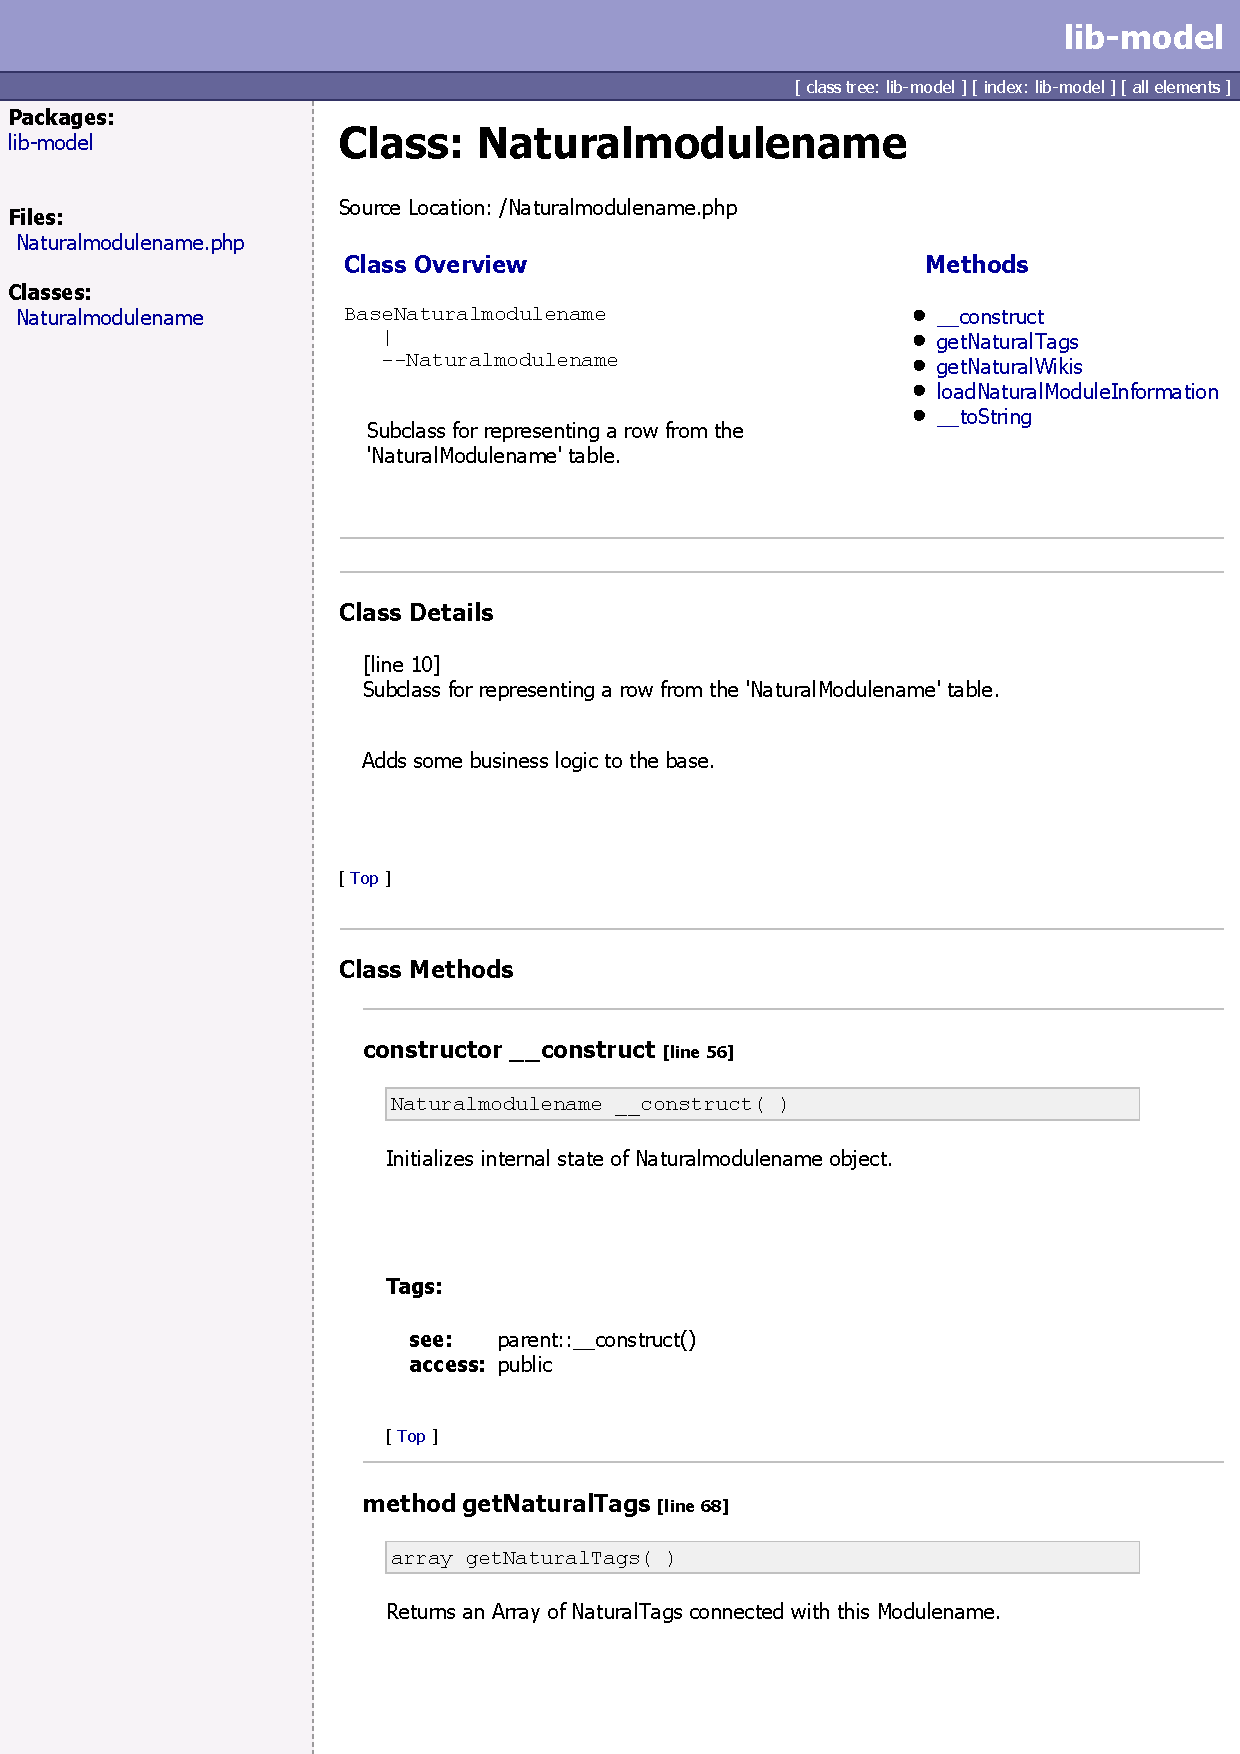
\includegraphics[page=1, width=0.9\textwidth]{doc.pdf}

\includegraphics[page=2, width=0.9\textwidth]{doc.pdf}
\end{center}

\clearpage
\subsection{Testfall und sein Aufruf auf der Konsole}
\label{app:Test}
\lstinputlisting[language=php, caption={Testfall in PHP}]{Listings/tests.php}
\clearpage
\begin{figure}[htb]
\centering
\includegraphicsKeepAspectRatio{testcase.jpg}{1}
\caption{Aufruf des Testfalls auf der Konsole}
\end{figure}


\subsection{Klasse: ComparedNaturalModuleInformation}
\label{app:CNMI}
Kommentare und simple Getter/Setter werden nicht angezeigt.
\lstinputlisting[language=php, caption={Klasse: ComparedNaturalModuleInformation}]{Listings/cnmi.php}
\clearpage

\subsection{Klassendiagramm}
\label{app:Klassendiagramm}
Klassendiagramme und weitere \acs{UML}-Diagramme kann man auch direkt mit \LaTeX{} zeichnen, siehe \zB \url{http://metauml.sourceforge.net/old/class-diagram.html}.
\begin{figure}[htb]
\centering
\includegraphicsKeepAspectRatio{Klassendiagramm.pdf}{1}
\caption{Klassendiagramm}
\end{figure}
\clearpage

\subsection{Benutzerdokumentation}
\label{app:BenutzerDoku}
Auszug aus der Benutzerdokumentation:

\begin{minipage}{0.5\textwidth}
\includegraphicsKeepAspectRatio{UebersichtDoku.png}{0.95}
\end{minipage}
\hfill
\begin{minipage}{0.5\textwidth}
    (1) zeigt den Namen des Sensors.Das davorstehende Icon zeigt die Art des Sensortyps. In diesem Fall ein Luftdrucksensor.

    (2) zeigt den aktuellsten Zählerstand

    (3) zeigt den aktuellsten Batteriestand

    (4) zeigt wann die letzten Daten geschickt wurden
\end{minipage}

\begin{minipage}{0.5\textwidth}
    (1) Sie können hier klicken um die Historie anzuzeigen

    (2) zeigt den aktuellsten Batteriestand in Prozent

    (3) Sie können den Knopf drücken um den Sensor als Favoriten zu markieren
\end{minipage}
\hfill
\begin{minipage}{0.5\textwidth}
    \hfill
    \includegraphicsKeepAspectRatio{DetailDoku.png}{0.95}
\end{minipage}

\begin{minipage}{0.5\textwidth}
\includegraphicsKeepAspectRatio{HistorieDoku.png}{0.95}
\end{minipage}
\hfill
\begin{minipage}{0.5\textwidth}
    (1) Sie können die Genauigkeit der Daten auswählen

    (2) zeigt den Wert des Vorzeitraums (Montag der letzten Woche)

    (3) zeigt einen Wert des aktuellen Zeitraums (Montag der aktuellen Woche)

    (4) zeigt den Wert des kompletten Zeitraums (komplette aktuelle Woche)

    (5) zeigt den Wert des kompletten Vorzeitraums (komplette letzte Woche)
\end{minipage}


\end{document}
